
\section{Experimental results}
\label{sec:experiments}

\subsection{Setup}
In order to asses the performance of our approach, we evaluate \FAMA on a wide range of domains. All tested domains are IPC domains that satisfy the \strips\ requirement~\cite{fox2003pddl2}, taken from the {\sc planning.domains} repository~\cite{muise2016planning}. Table \ref{tab:domain_features} compiles the features of the thirteen domains used in the experiments. From left to right, the columns report the name of the domain, number of actions, number of predicates, maximum arity of the actions, and maximum arity of the predicates. These are all features which affect the size of $P_\Lambda$ and, hence, have an impact on the complexity of the learning task. As can be seen in table \ref{tab:domain_features}, the selected domains range from simple ones, such as \emph{blocks} and \emph{visitall}, to complex ones, like \emph{floortile} and \emph{satellite}, with higher number of actions and predicates and with higher arity.

Following, we explain the details of our experimental setup:

\begin{itemize}

\item {\bf Plan traces}. For each domain, we have generated 10 plan traces with 10 actions/intermediate states each using random walks. Depending on the experiment, these traces may be used for training or testing, so more details will be provided later.

\item {\bf Planner}. The classical planner we use to solve the instances that result from our compilations is {\sc Madagascar}~\cite{rintanen2014madagascar}. We use {\sc Madagascar} for two reasons: 1) its ability to deal with planning instances populated with dead-ends, and 2) when the length of the plan traces is known (\FO action sequences or \FO state trajectories), the horizon of the solution plan is also known and can be solved as a NP-complete problem. This is because, SAT-based planners can apply the actions for programming preconditions in parallel during a single planning step (and the same for actions programming effects) because these actions do not interact. Hence, we know that the programming prefix of the solution plan can be solved in two steps, independently of the number of programming actions applied.

\item {\bf Machine}. All experiments are run on an Intel Core i5 3.50 GHz x 4 with 16 GB of RAM.

\item {\bf Reproducibility}. We make fully available the compilation source code, the evaluation scripts and the used benchmarks at this repository {\em https://github.com/sjimenezgithub/strips-learning} so any experimental data reported in the paper is fully reproducible.
\end{itemize}

\begin{table}[hbt!]
		\begin{center}
			\begin{tabular}{l|c|c|c|c|}	
				& \multicolumn{4}{c|}{Domain features}\\ \cline{2-5}
				Domain & \# actions & \# predicates & max action arity & max predicate arity  \\
				\hline
				Blocks & 4 & 5 & 2 & 2  \\
				Driverlog & 6 & 5 & 4 & 2  \\
				Ferry & 3 & 5 & 2 & 2  \\
				Floortile & 7 & 10 & 4 & 2  \\
				Grid & 5 & 9 & 4 & 2  \\
				Gripper & 3 & 4 & 3 & 2  \\
				Hanoi & 1 & 3 & 3 & 2  \\
				Miconic & 4 & 6 & 2 & 2  \\
				Npuzzle & 1 & 3 & 3 & 2  \\
				Parking & 4 & 5 & 3 & 2  \\
				Satellite & 5 & 8 & 4 & 2  \\
				Transport & 3 & 5 & 5 & 2  \\
				Visitall & 1 & 3 & 2 & 2  \\
			\end{tabular}
		\end{center}
	\caption{\small Feature description of the 13 domains used in the experiments.}
	\label{tab:domain_features}	
\end{table}

\subsection{Impact of the size of the input knowledge}
In our first experiment, we evaluate how the size of the input knowledge, i.e., $\left|\mathcal{T}\right|$ affects \FAMA. The experiment consists in increasing the size of $\mathcal{T}$ from 1 to 10, and analyze the evolution of the computation time as well as the quality of the learned models. 
Our goals with this experiment are:
\begin{enumerate}
	\item Identify the amount of input required by \FAMA to learn good models,
	\item Evaluate the scalability of \FAMA wrt the input size which, as stated in section \ref{properties}, is one of the limiting factors of our approach.
\end{enumerate} 

With this in mind we have defined two case studies:
\begin{itemize}
	\item \textbf{\FO action sequence and \PO state trajectory}: This is the typical case solved by most approaches, which corresponds to a NP-complete scenario. We are assuming a degree of observability of 10\% for the state trajectory, meaning that each literal of a state has a 10\% chance of being observed.
	\item  \textbf{\NO action sequence and \NO state trajectory}: This is a PSPACE-complete scenario where both the action sequence and state trajectory are completely empty and only initial and final states are observed, i.e., $\tau = \tup{s_0, s_m}, \forall \tau \in \mathcal{T}$.
\end{itemize}

\begin{figure}[hbt!]
	\centering
	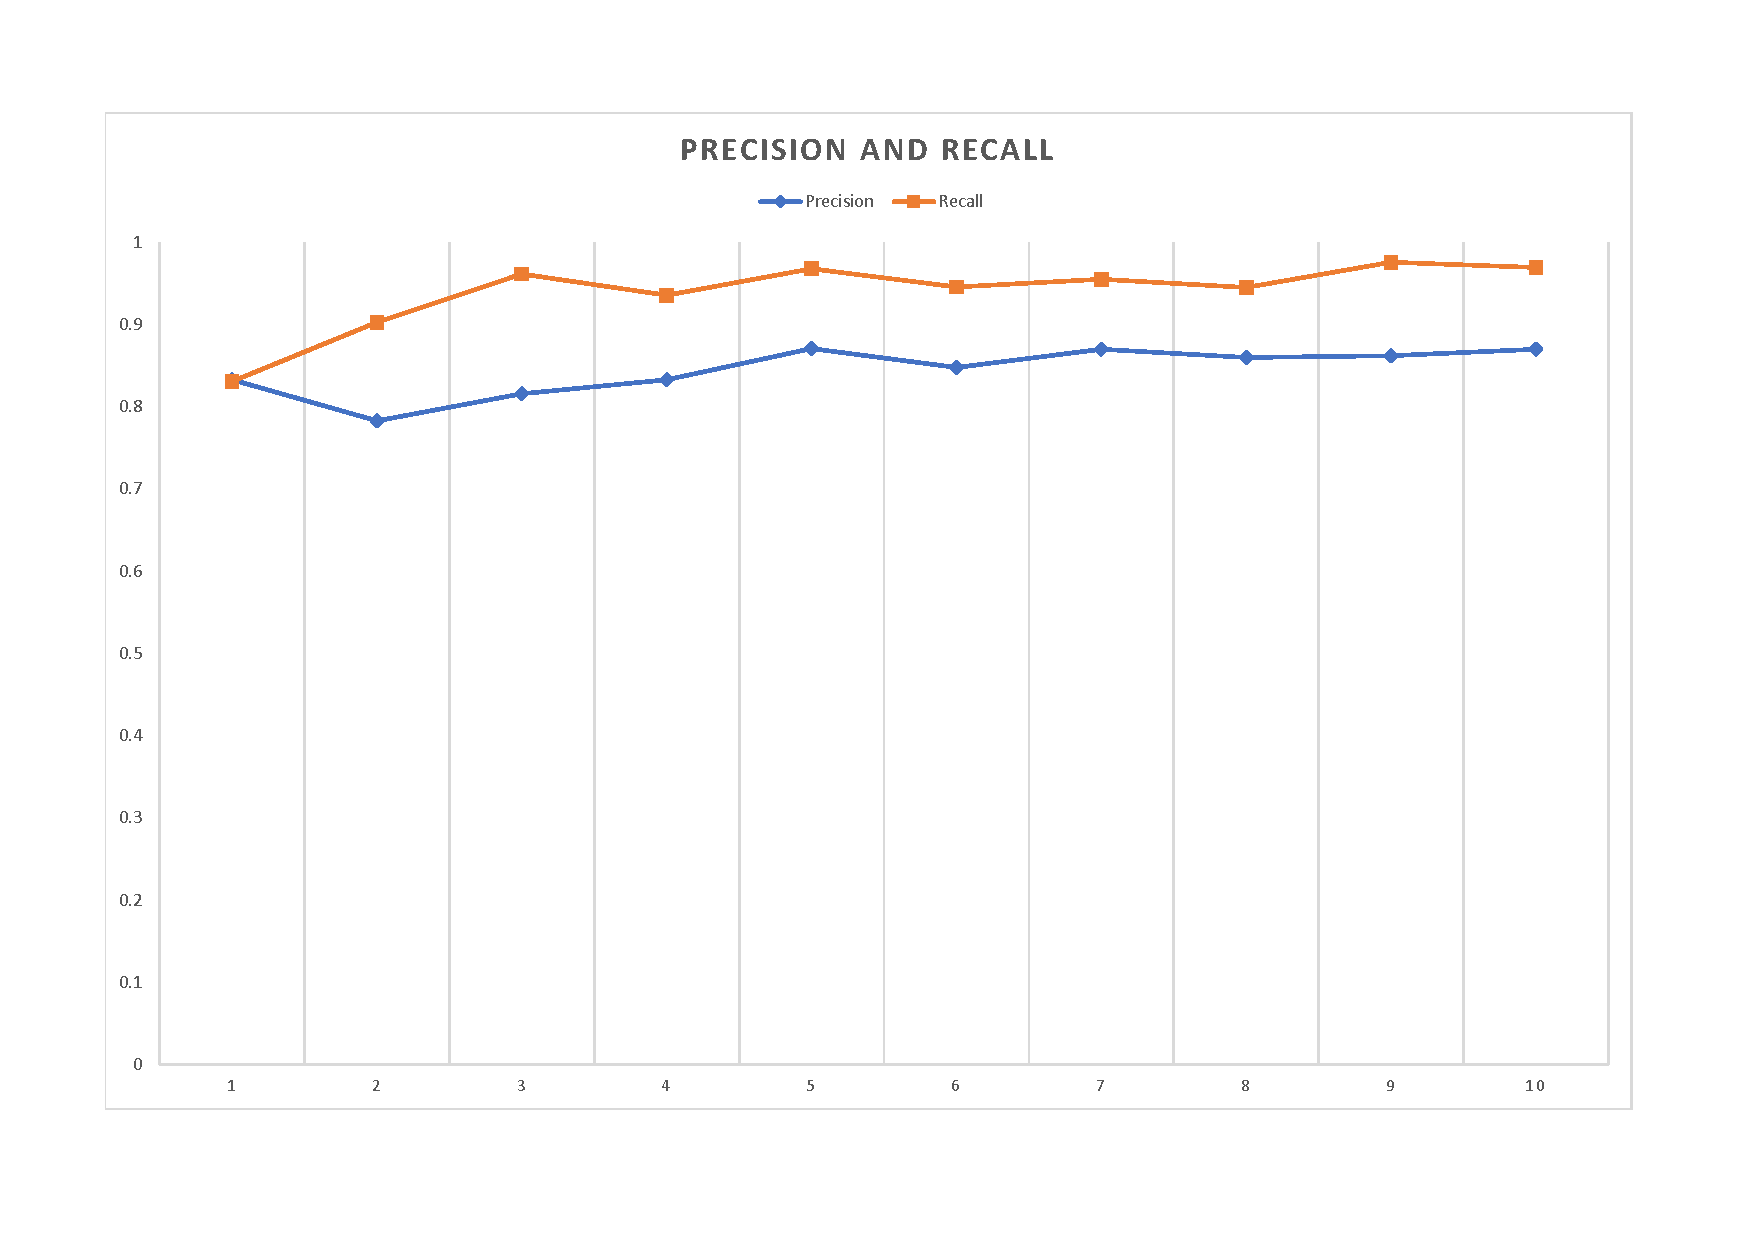
\includegraphics[width=0.8\linewidth]{figures/input_size_100_10_precision.pdf}
	\caption{Evaluation of the impact of the input size on the quality of the learned models when learning from plan traces with \FO action sequences and \PO state trajectories with 10\% observability}
\end{figure}

\begin{figure}[hbt!]
	\centering
	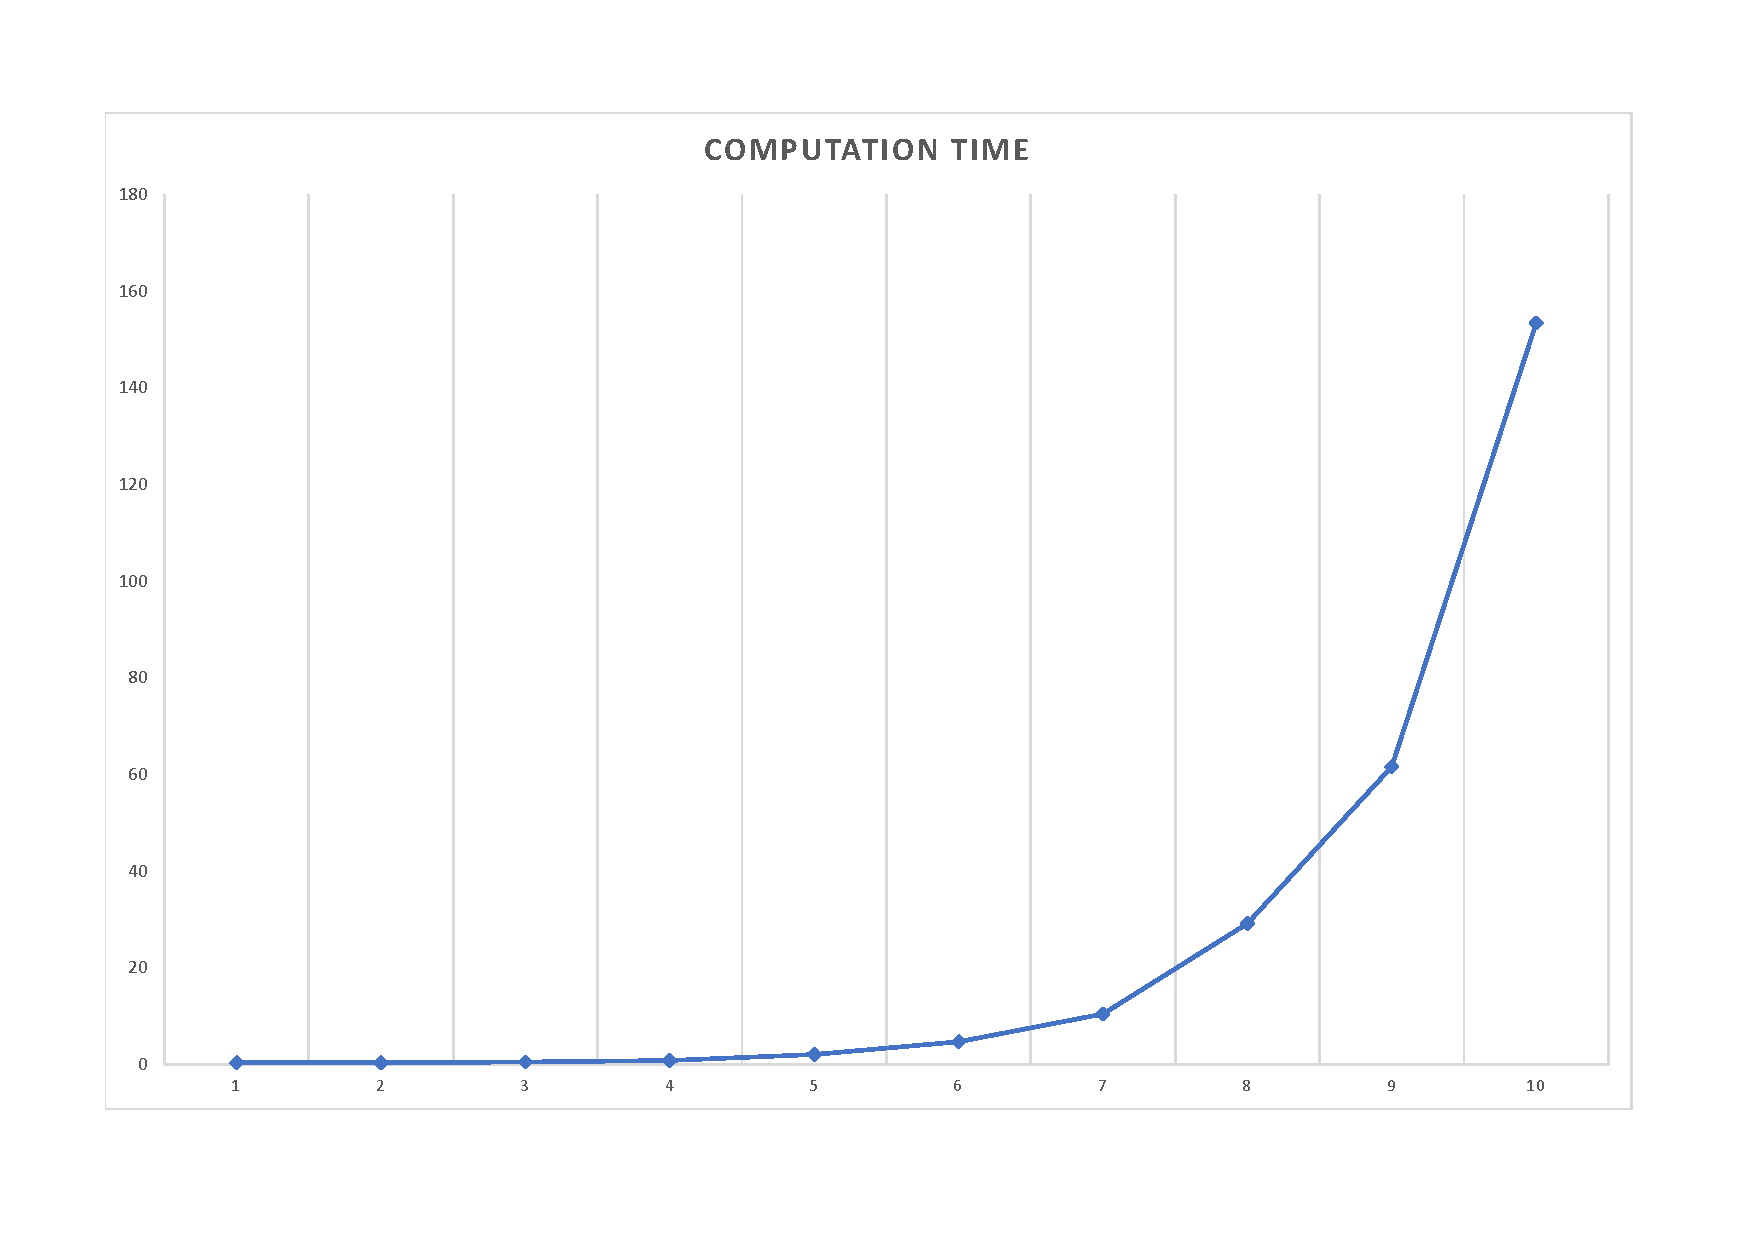
\includegraphics[width=0.8\linewidth]{figures/input_size_100_10_time.pdf}
	\caption{Evaluation of the impact of the input size on the computation time when learning from plan traces with \FO action sequences and \PO state trajectories with 10\% observability}
\end{figure}

\begin{figure}[hbt!]
	\centering
	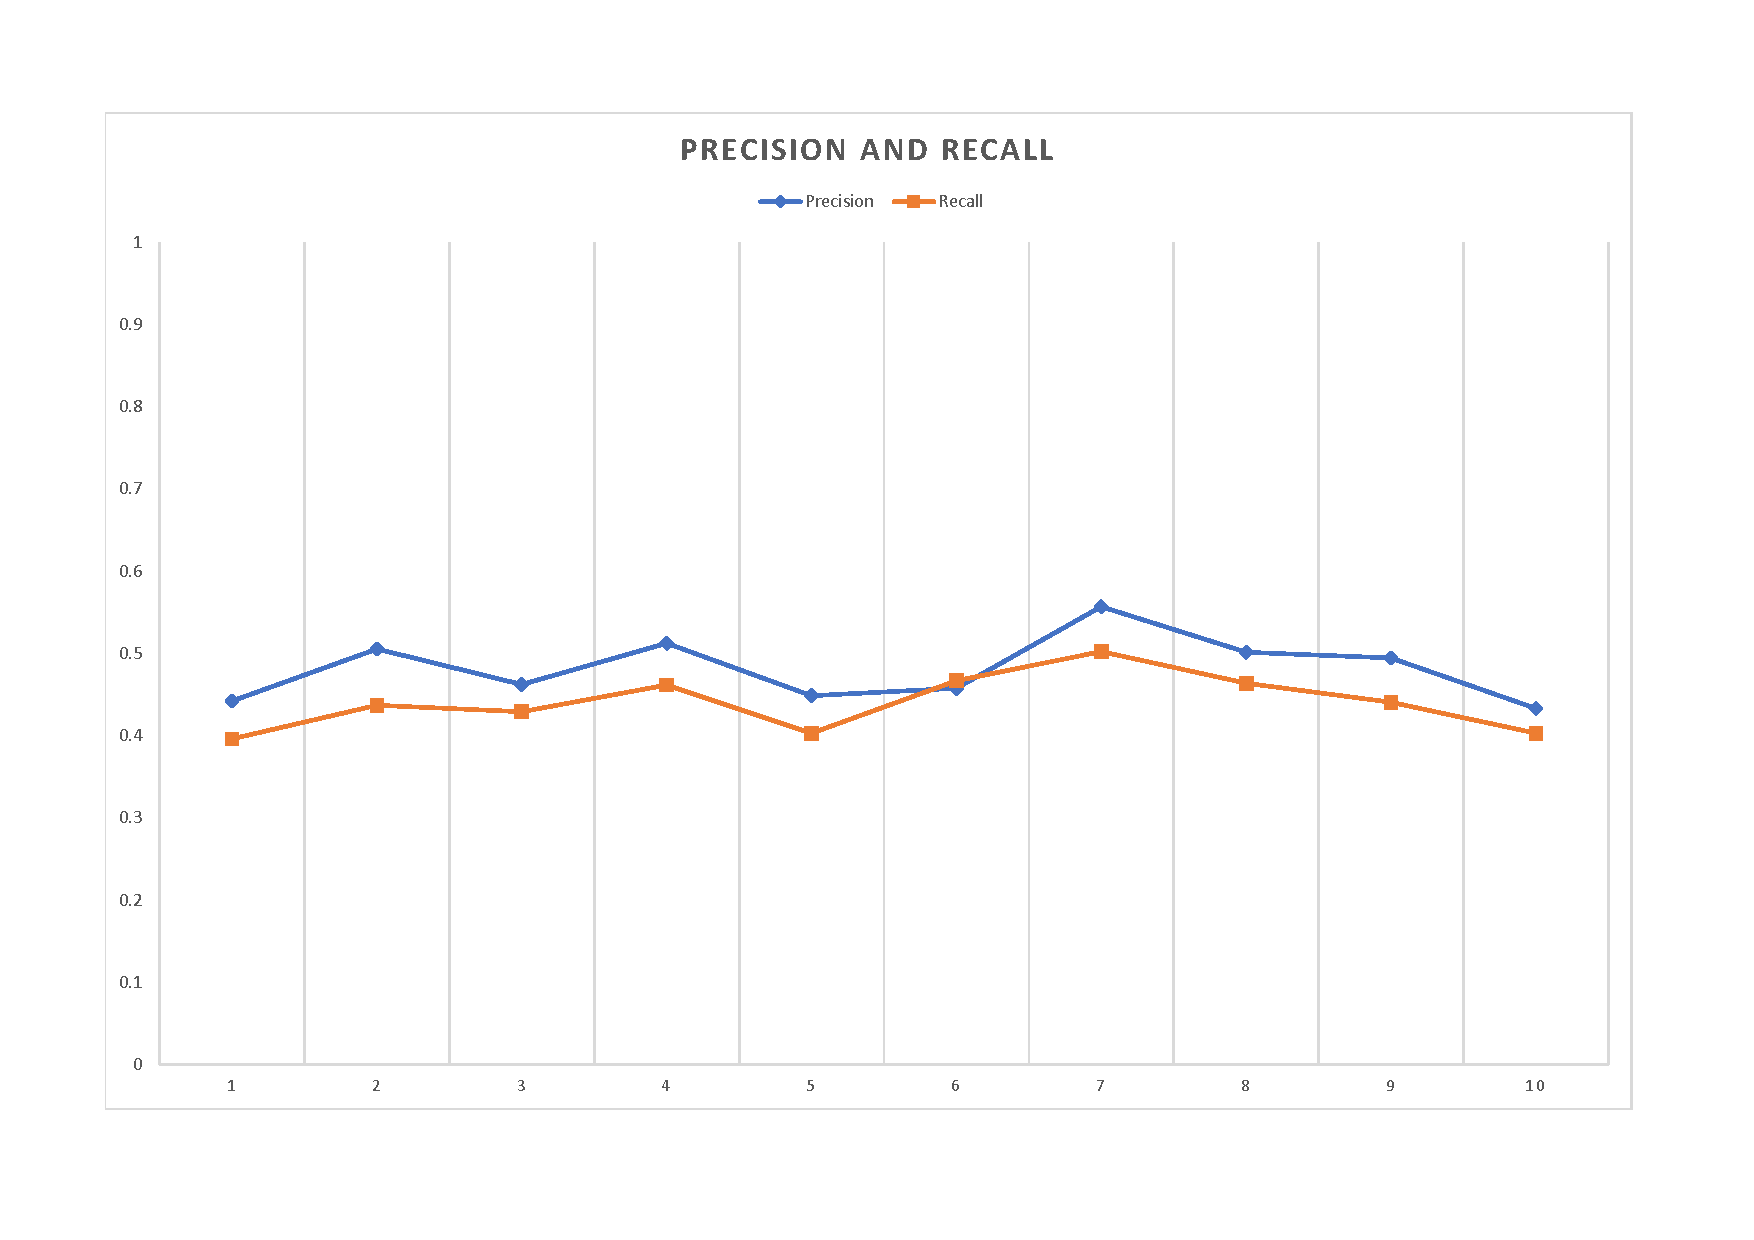
\includegraphics[width=0.8\linewidth]{figures/input_size_0_0_precision.pdf}
	\caption{Evaluation of the impact of the input size on the quality of the learned models when learning from plan traces with \NO action sequences and \NO state trajectories}
\end{figure}

\begin{figure}[hbt!]
	\centering
	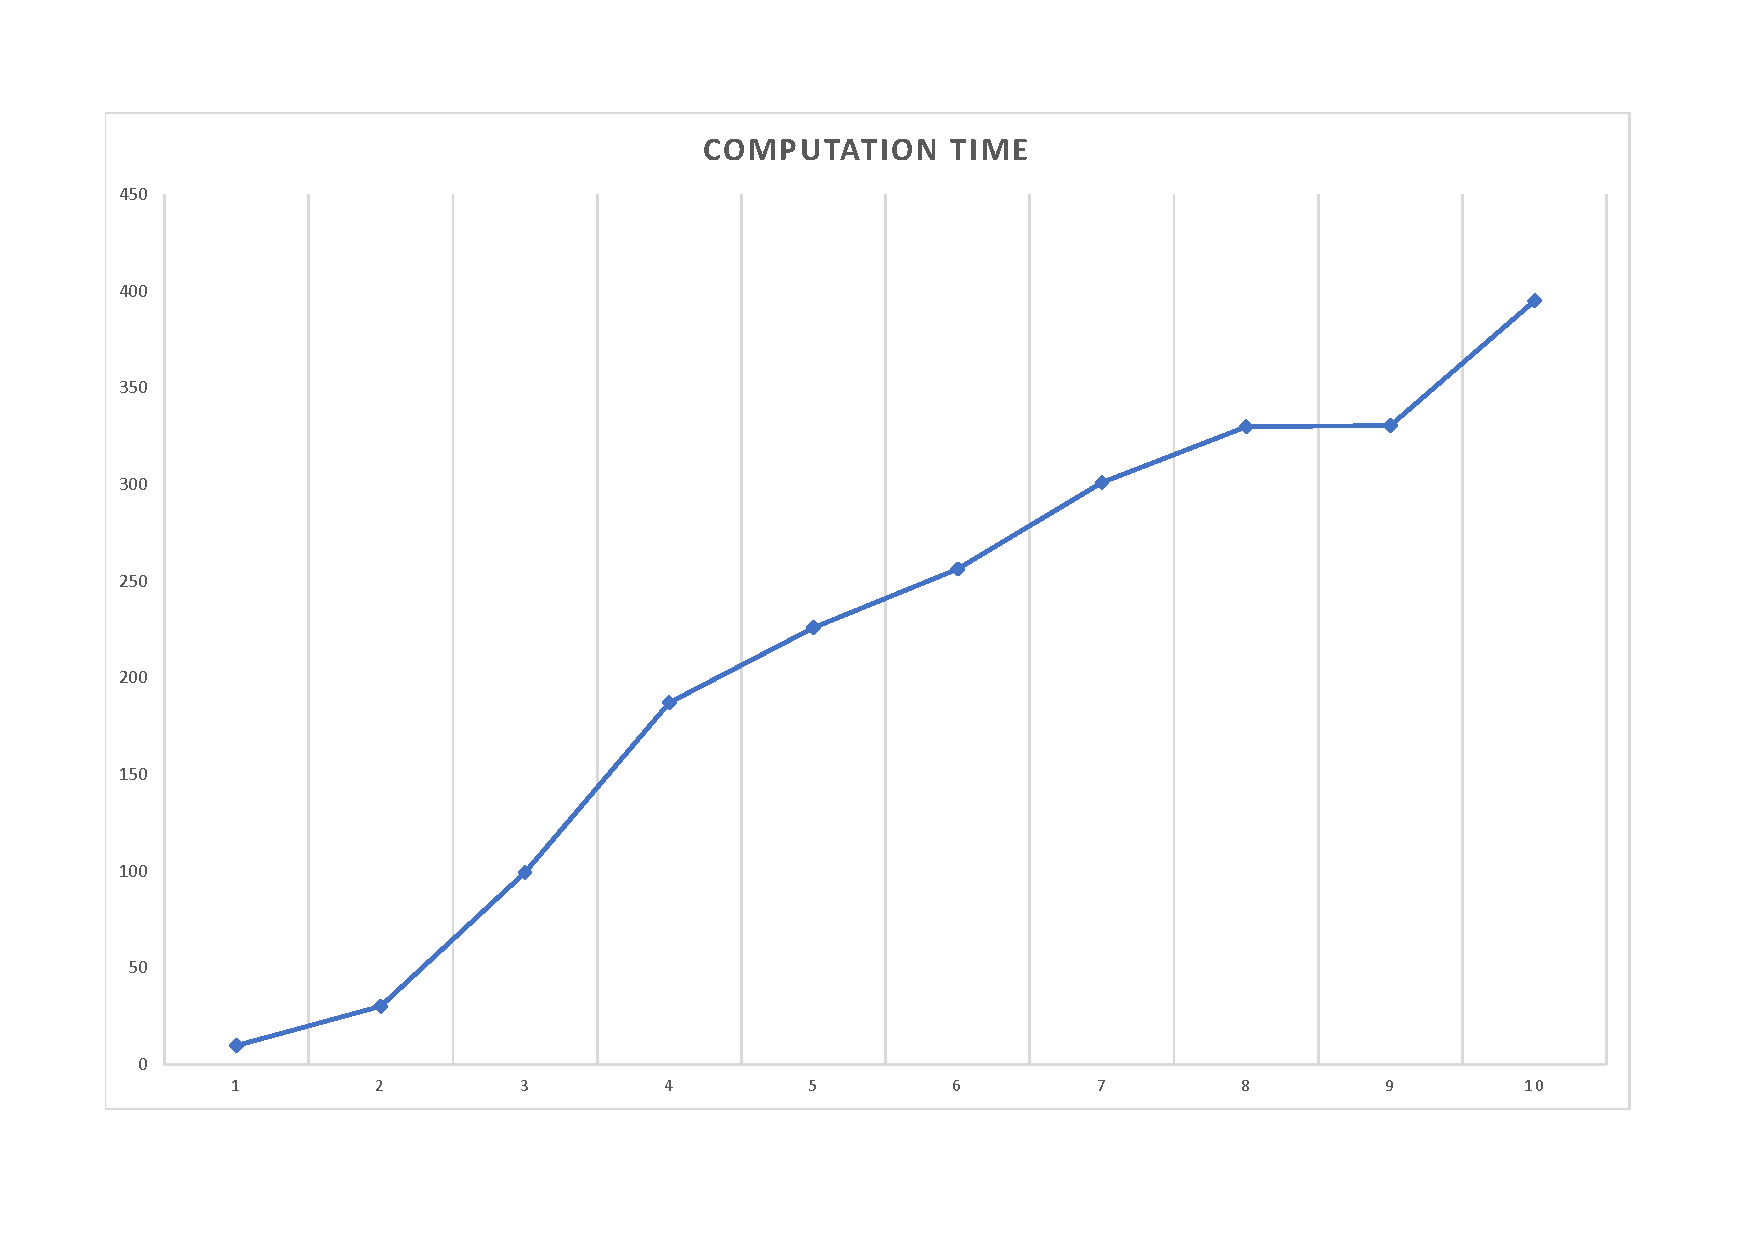
\includegraphics[width=0.8\linewidth]{figures/input_size_0_0_time.pdf}
	\caption{Evaluation of the impact of the input size on the computation time when learning from plan traces with \NO action sequences and \NO state trajectories}
\end{figure}

\subsection{Comparison with \ARMS}
Here we compare the performance of \FAMA to that of \ARMS, one of the most well-known approaches in the action model acquisition field. \ARMS works under the assumption of plan traces with \FO action sequences and \NO state trajectories, so we will also adopt this assumption. In more detail, we define a \emph{degree of observability} $\sigma$ for the state trajectory, ranging from 0\% to 100\%, that measures the probability of observing a literal, and evaluate both approaches as $\sigma$ increases. Note that when $\sigma = 0$ we have a \NO state trajectory and when $\sigma=100$ we have a \FO state trajectory, all cases in-between correspond to the \PO scenario.

\begin{figure}[hbt!]
	\centering
	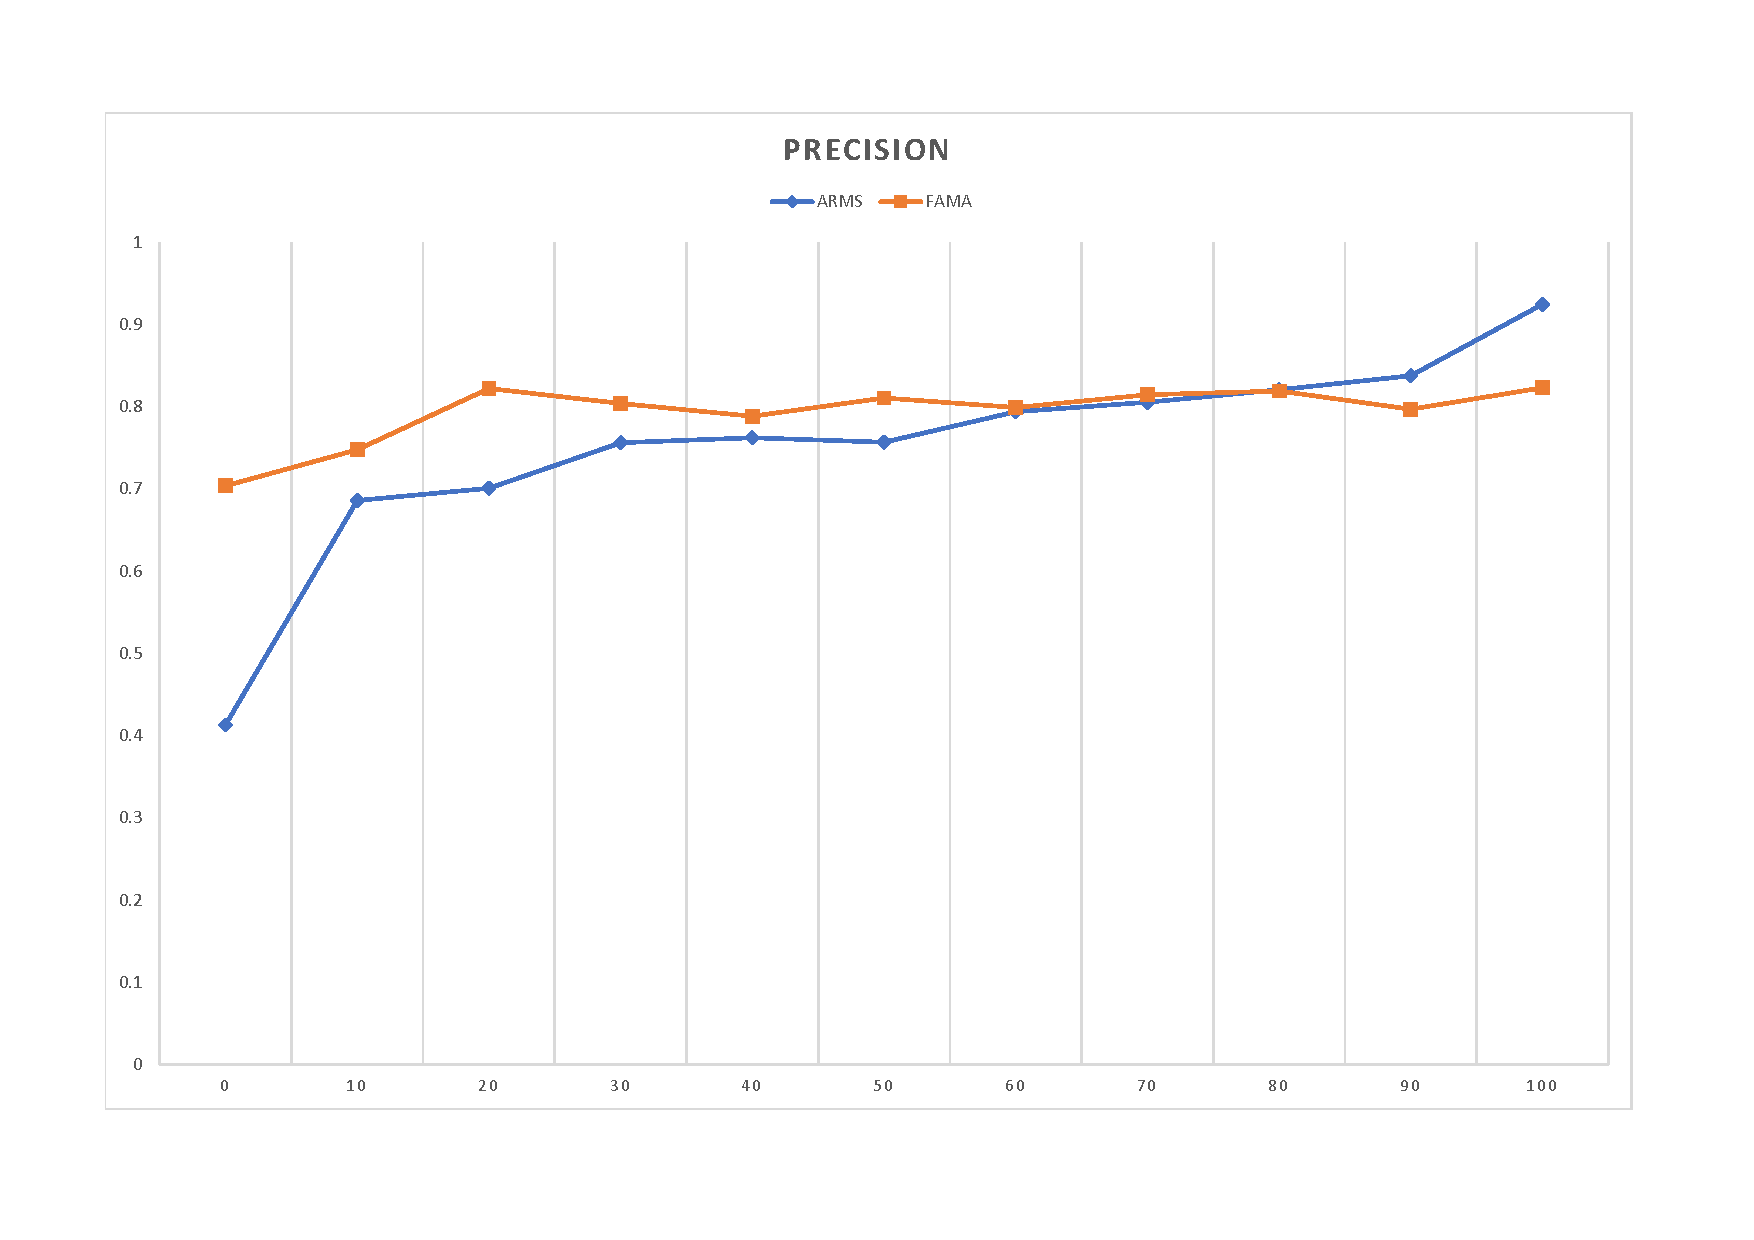
\includegraphics[width=.8\linewidth]{figures/comparison_precision.pdf}
	\caption{Precision comparison between \FAMA and \ARMS}
	\label{fig:comparison_precision}
\end{figure}

\begin{figure}[hbt!]
	\centering
	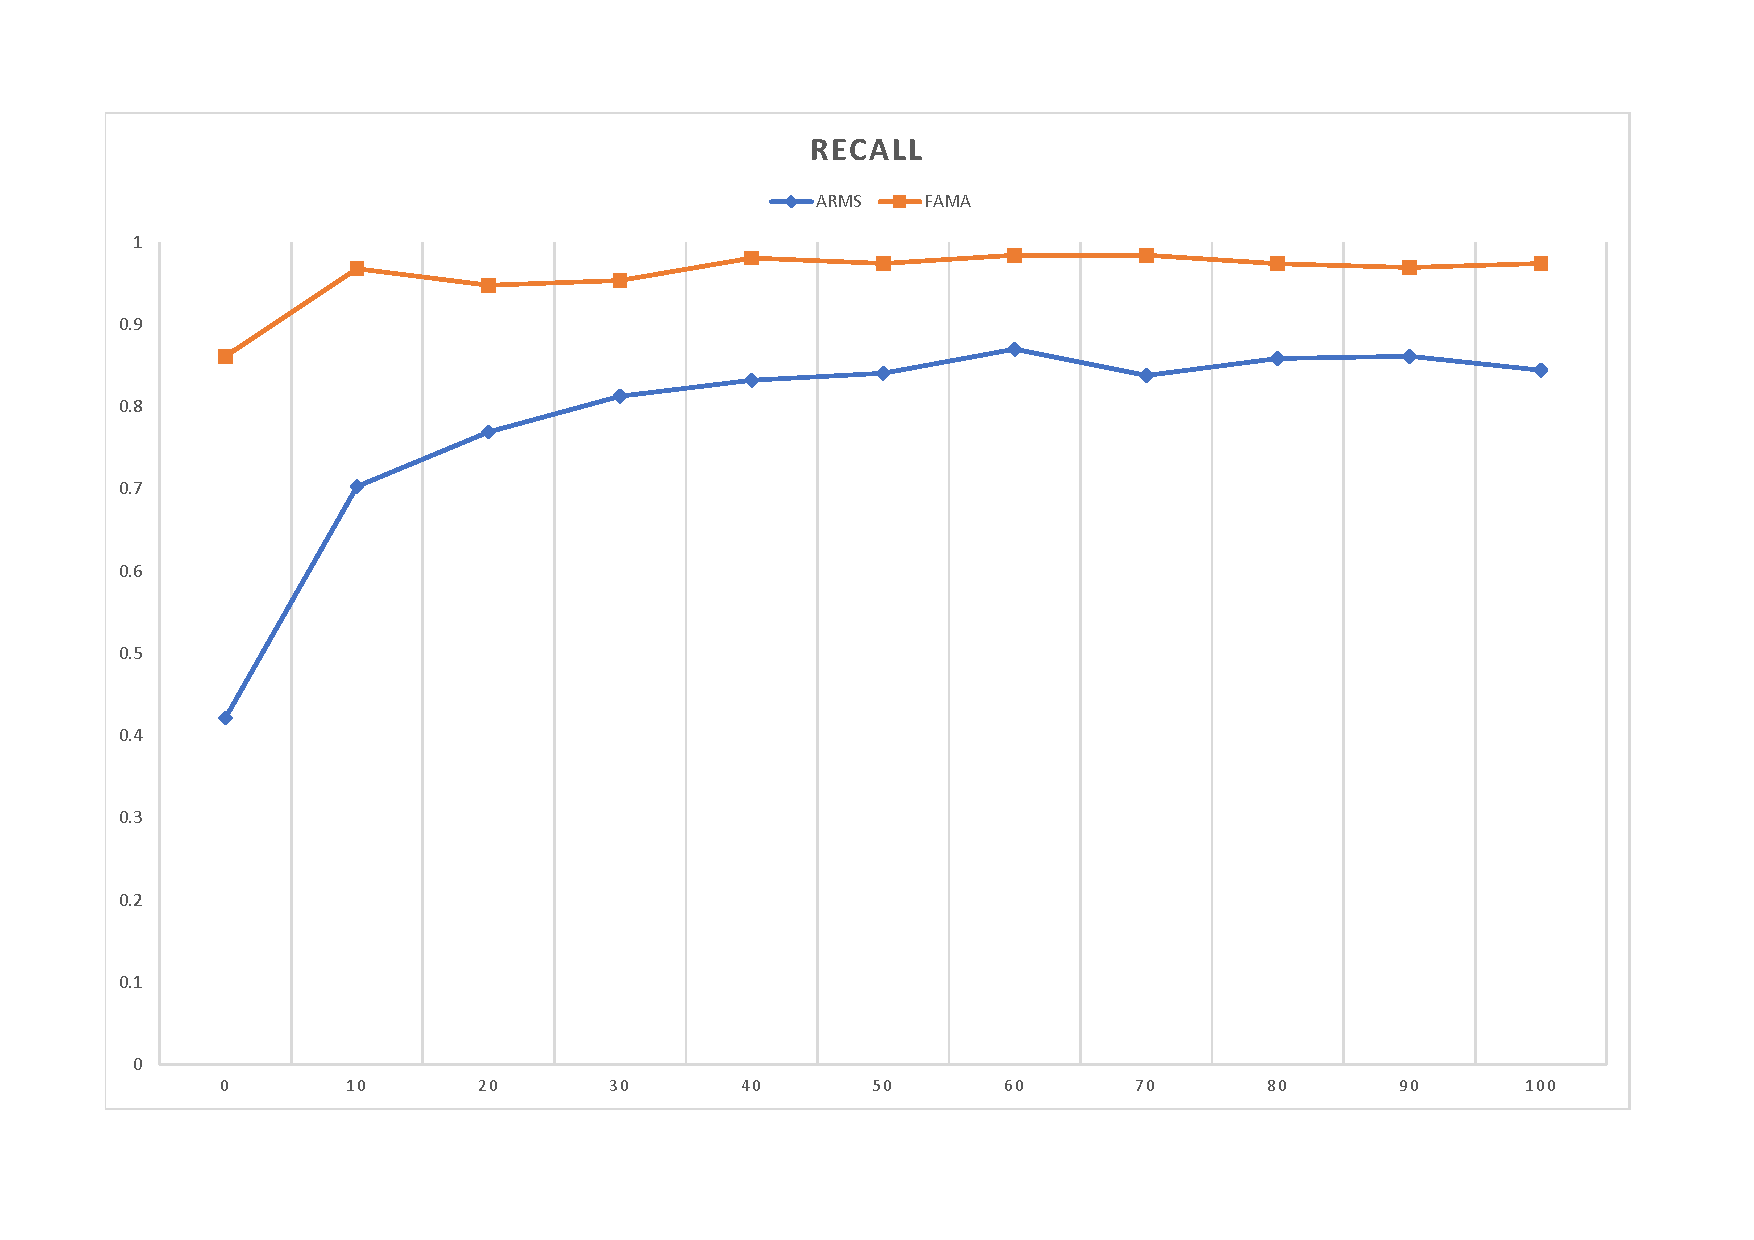
\includegraphics[width=.8\linewidth]{figures/comparison_recall.pdf}
	\caption{Recall comparison between \FAMA and \ARMS}
	\label{fig:comparison_recall}
\end{figure}

Figures \ref{fig:comparison_precision} and \ref{fig:comparison_recall} compare \FAMA and \ARMS in terms of precision and recall. The horizontal axis represents the degree of observability, while the vertical axis show the average precision (figure \ref{fig:comparison_precision}) or recall (figure \ref{fig:comparison_recall}) computed over the 13 tested domains.

\subsection{Experiments with minimal input knowledge}
In the previous experiments we have given a general view of the performance of \FAMA under different conditions. So far, experiments have shown that \FAMA is able to learn with very small amounts of input knowledge, be it due to low observability or few training samples. In this section we want to take a closer look at the action models learned from minimal input knowledge. To that end, we will limit the input to only 2 plan traces and analyze the results under different levels of observability.

All tables in this section (tables \ref{tab:results_minimum_0_0}, \ref{tab:results_minimum_0_20}) follow the same structure. In these tables precision ({\bf P}) and recall ({\bf R}) are computed separately for the preconditions ({\bf Pre}), positive effects ({\bf Add}) and negative Effects ({\bf Del}), and also globally ({\bf Global}). The last column reports the computation time in seconds needed to obtain the learned models. We can observe that identifying static predicates leads to models with better precondition {\em recall}. This fact evidences that many of the missing preconditions corresponded to static predicates because there is no incentive to learn them as they always hold~\cite{gregory2015domain}.

\begin{table}[hbt!]
		\begin{center}
			
			\begin{tabular}{l|l|l|l|l|l|l||l|l|l|}
				& \multicolumn{2}{|c|}{\bf Pre} & \multicolumn{2}{|c|}{\bf Add} & \multicolumn{2}{|c||}{\bf Del} & \multicolumn{2}{|c|}{\bf Global} & \\ \cline{2-9}			
				& \multicolumn{1}{|c|}{\bf P} & \multicolumn{1}{|c|}{\bf R} & \multicolumn{1}{|c|}{\bf P} & \multicolumn{1}{|c|}{\bf R} & \multicolumn{1}{|c|}{\bf P} & \multicolumn{1}{|c||}{\bf R} &  \multicolumn{1}{|c|}{\bf P} & \multicolumn{1}{|c|}{\bf R} & {\bf Time} \\
				\hline
				blocks & 0.6 & 0.67 & 0.29 & 0.22 & 0.75 & 0.33 & 0.55 & 0.41& 0.22 \\ % [(u'pick-up', u'pick-up', 1), (u'put-down', u'put-down', 1), (u'stack', u'unstack', 2, 1), (u'unstack', u'stack', 2, 1)]
				driverlog & 0.45 & 0.36 & 0.36 & 0.57 & 0.17 & 0.14 & 0.33 & 0.36& 1.59 \\ % [(u'load-truck', u'walk', 2, 1, 3), (u'unload-truck', u'disembark-truck', 1, 2, 3), (u'board-truck', u'unload-truck', 1, 2, 3), (u'disembark-truck', u'board-truck', 1, 2, 3), (u'walk', u'walk', 1, 2, 3), (u'drive-truck', u'drive-truck', 1, 2, 3, 4)]
				ferry & 0.6 & 0.43 & 0.4 & 0.5 & 0.5 & 0.5 & 0.5 & 0.48& 0.51 \\ % [(u'sail', u'sail', 1, 2), (u'board', u'board', 1, 2), (u'debark', u'debark', 1, 2)]
				floor-tile & 0.67 & 0.45 & 0.6 & 0.55 & 0.88 & 0.64 & 0.71 & 0.55& 359.43 \\ % [(u'change-color', u'change-color', 1, 2, 3), (u'up', u'up', 1, 3, 2), (u'down', u'down', 1, 3, 2), (u'right', u'right', 1, 2, 3), (u'left', u'left', 1, 2, 3), (u'paint-up', u'paint-up', 1, 3, 2, 4), (u'paint-down', u'paint-down', 1, 2, 3, 4)]
				grid & 0.37 & 0.41 & 0.5 & 0.71 & 0.33 & 0.43 & 0.4 & 0.52& 81.71 \\ % [(u'move', u'move', 1, 2), (u'pickup', u'putdown', 1, 2), (u'putdown', u'pickup', 1, 2), (u'pickup-and-loose', u'pickup-and-loose', 1, 3, 2), (u'unlock', u'unlock', 1, 2, 3, 4)]
				gripper-strips & 0.8 & 0.67 & 0.6 & 0.75 & 0.8 & 1.0 & 0.73 & 0.81& 0.09 \\ % [(u'move', u'move', 1, 2), (u'pick', u'pick', 1, 2, 3), (u'drop', u'drop', 1, 2, 3)]
				hanoi & 1.0 & 0.5 & 0.5 & 0.5 & 1.0 & 1.0 & 0.83 & 0.67& 0.87 \\ % [(u'move', u'move', 1, 3, 2)]
				miconic & 0.67 & 0.22 & 0.67 & 0.5 & 1.0 & 0.67 & 0.78 & 0.46& 0.25 \\ % [(u'board', u'depart', 1, 2), (u'depart', u'board', 1, 2), (u'up', u'up', 2, 1), (u'down', u'down', 1, 2)]
				n-puzzle & 0.0 & 0.0 & 0.0 & 0.0 & 0.0 & 0.0 & 0.0 & 0.0& 0.47 \\ % [(u'move', u'move', 1, 2, 3)]
				parking & 0.64 & 0.5 & 0.63 & 0.56 & 0.5 & 0.44 & 0.59 & 0.5& 12.56 \\ % [(u'move-curb-to-curb', u'move-curb-to-curb', 1, 3, 2), (u'move-curb-to-car', u'move-curb-to-car', 3, 2, 1), (u'move-car-to-curb', u'move-car-to-curb', 2, 1, 3), (u'move-car-to-car', u'move-car-to-car', 1, 3, 2)]
				satellite & 0.38 & 0.21 & 0.5 & 0.6 & 0.75 & 0.75 & 0.54 & 0.52& 1.86 \\ % [(u'switch-on', u'switch-on', 1, 2), (u'switch-off', u'switch-off', 1, 2), (u'turn-to', u'turn-to', 1, 2, 3), (u'calibrate', u'calibrate', 1, 2, 3), (u'take-image', u'take-image', 1, 2, 3, 4)]
				transport & 0.43 & 0.3 & 0.4 & 0.4 & 0.0 & 0.0 & 0.28 & 0.23& 0.88 \\ % [(u'drive', u'drive', 1, 3, 2), (u'pick-up', u'pick-up', 1, 2, 3, 4, 5), (u'drop', u'drop', 1, 2, 3, 4, 5)]
				grid-visit-all & 0.0 & 0.0 & 1.0 & 0.5 & 0.0 & 0.0 & 0.33 & 0.17& 1.54 \\ % [(u'move', u'move', 2, 1)]			
				\hline
				\bf & 0.51& 0.36 & 0.50 & 0.49 & 0.51 & 0.45 & 0.51 & 0.44 & 35.54 \\
			\end{tabular}
			
		\end{center}
	\caption{\small {\em Precision} and {\em recall} scores for learning tasks with \NO action sequences and \NO state trajectories}
	\label{tab:results_minimum_0_0}
\end{table}


\begin{table}[hbt!]
	\begin{center}
		
		\begin{tabular}{l|l|l|l|l|l|l||l|l|l|}
			& \multicolumn{2}{|c|}{\bf Pre} & \multicolumn{2}{|c|}{\bf Add} & \multicolumn{2}{|c||}{\bf Del} & \multicolumn{2}{|c|}{\bf Global} & \\ \cline{2-9}			
			& \multicolumn{1}{|c|}{\bf P} & \multicolumn{1}{|c|}{\bf R} & \multicolumn{1}{|c|}{\bf P} & \multicolumn{1}{|c|}{\bf R} & \multicolumn{1}{|c|}{\bf P} & \multicolumn{1}{|c||}{\bf R} &  \multicolumn{1}{|c|}{\bf P} & \multicolumn{1}{|c|}{\bf R} & {\bf Time} \\
			\hline
			blocks & 0.78 & 0.78 & 0.6 & 0.67 & 0.8 & 0.44 & 0.73 & 0.63& 0.27 \\ % [(u'pick-up', u'pick-up', 1), (u'put-down', u'put-down', 1), (u'stack', u'unstack', 1, 2), (u'unstack', u'stack', 2, 1)]
			driverlog & 0.5 & 0.07 & 0.18 & 0.57 & 0.0 & 0.0 & 0.23 & 0.21& 1.01 \\ % [(u'load-truck', u'walk', 2, 1, 3), (u'unload-truck', u'board-truck', 1, 2, 3), (u'board-truck', u'unload-truck', 1, 2, 3), (u'disembark-truck', u'disembark-truck', 1, 2, 3), (u'walk', u'walk', 1, 2, 3), (u'drive-truck', u'drive-truck', 1, 2, 3, 4)]
			ferry & 0.83 & 0.71 & 0.75 & 0.75 & 0.8 & 1.0 & 0.79 & 0.82& 0.37 \\ % [(u'sail', u'sail', 1, 2), (u'board', u'debark', 1, 2), (u'debark', u'board', 1, 2)]
			floor-tile & 0.68 & 0.59 & 0.62 & 0.73 & 0.75 & 0.55 & 0.68 & 0.62& 186.92 \\ % [(u'change-color', u'change-color', 1, 3, 2), (u'up', u'right', 1, 2, 3), (u'down', u'up', 1, 3, 2), (u'right', u'down', 1, 2, 3), (u'left', u'left', 1, 3, 2), (u'paint-up', u'paint-down', 1, 2, 3, 4), (u'paint-down', u'paint-up', 1, 2, 3, 4)]
			grid & 0.46 & 0.35 & 0.25 & 0.43 & 0.63 & 0.71 & 0.45 & 0.5& 107.9 \\ % [(u'move', u'move', 2, 1), (u'pickup', u'pickup', 1, 2), (u'putdown', u'putdown', 1, 2), (u'pickup-and-loose', u'pickup-and-loose', 1, 2, 3), (u'unlock', u'unlock', 1, 2, 3, 4)]
			gripper-strips & 0.57 & 0.67 & 0.67 & 0.5 & 1.0 & 0.75 & 0.75 & 0.64& 0.06 \\ % [(u'move', u'move', 1, 2), (u'pick', u'drop', 1, 2, 3), (u'drop', u'pick', 1, 2, 3)]
			hanoi & 0.6 & 0.75 & 1.0 & 1.0 & 1.0 & 1.0 & 0.87 & 0.92& 1.09 \\ % [(u'move', u'move', 1, 3, 2)]
			miconic & 1.0 & 0.11 & 0.33 & 0.5 & 1.0 & 0.33 & 0.78 & 0.31& 0.17 \\ % [(u'board', u'board', 1, 2), (u'depart', u'up', 1, 2), (u'up', u'depart', 1, 2), (u'down', u'up', 2, 1)]
			n-puzzle & 0.75 & 1.0 & 1.0 & 1.0 & 1.0 & 1.0 & 0.92 & 1.0& 2.5 \\ % [(u'move', u'move', 1, 2, 3)]
			parking & 0.45 & 0.36 & 0.4 & 0.44 & 0.63 & 0.56 & 0.49 & 0.45& 5.87 \\ % [(u'move-curb-to-curb', u'move-curb-to-curb', 1, 3, 2), (u'move-curb-to-car', u'move-curb-to-car', 1, 2, 3), (u'move-car-to-curb', u'move-car-to-car', 2, 1, 3), (u'move-car-to-car', u'move-car-to-car', 3, 1, 2)]
			satellite & 0.67 & 0.43 & 0.25 & 0.4 & 0.29 & 0.5 & 0.4 & 0.44& 1.34 \\ % [(u'switch-on', u'switch-off', 1, 2), (u'switch-off', u'switch-on', 1, 2), (u'turn-to', u'turn-to', 1, 2, 3), (u'calibrate', u'calibrate', 1, 2, 3), (u'take-image', u'take-image', 1, 2, 3, 4)]
			transport & 0.33 & 0.1 & 0.4 & 0.4 & 0.0 & 0.0 & 0.24 & 0.17& 1.14 \\ % [(u'drive', u'drive', 1, 2, 3), (u'pick-up', u'pick-up', 1, 2, 3, 4, 5), (u'drop', u'drop', 1, 2, 3, 4, 5)]
			grid-visit-all & 0.5 & 0.5 & 1.0 & 1.0 & 1.0 & 1.0 & 0.83 & 0.83& 1.08 \\ % [(u'move', u'move', 2, 1)]
			
			\hline
			\bf & 0.62 & 0.49 & 0.57 & 0.65 & 0.68 & 0.60 & 0.63 & 0.58	& 23.82	 \\
		\end{tabular}
		
	\end{center}
	\caption{\small {\em Precision} and {\em recall} scores for learning tasks with \NO action sequences and \PO state trajectories with 20\% observability}
	\label{tab:results_minimum_0_20}
\end{table}

%Remarkably, the overall \emph{precision} is now $0.98$, which means that the contents of the learned models is highly reliable. The value of \emph{recall}, 0.87, is an indication that the learned models still miss some information (preconditions are again the component more difficult to be fully learned). Overall, the results confirm the previous trend: the more input knowledge of the task, the better the models and the less planning time. Additionally, the solution plans required for this task are smaller because it is only necessary to program half of the actions (the other half are included in the input knowledge $\mathcal{M}$). {\em Visitall} and {\em Hanoi} are excluded from this evaluation because they only contain one action schema.



%Here we evaluate our approach with learning tasks of the kind $\Lambda=\tup{\mathcal{M},\Psi,\mathcal{T}}$, where the action of the executed plans are not available but the initial and goal states are known. When input plans are not available, the planner must not only compute the action models but also the plans that satisfy the input observations. Table~\ref{tab:results_states} and ~\ref{tab:time_states} summarize the results obtained for this using static predicates and partially specified models. Values for the {\em Zenotravel} and {\em Grid} domains are not reported because {\sc Madagascar} was not able to solve the corresponding planning tasks within a 1000 sec. time bound. The values of \emph{precision} and \emph{recall} are significantly lower than in Table ~\ref{tab:results_plans}. Given that the learning hypothesis space is now fairly under-constrained, actions can be reformulated and still be compliant with the inputs (e.g. the {\em blocksworld} operator {\small\tt stack} can be {\em learned} with the preconditions and effects of the {\small\tt unstack} operator and vice versa). We tried to minimize this effect with the additional input knowledge (static predicates and partially specified action models) and yet the results are below the scores obtained when learning from labeled plans.

%To give an insight of the actual quality of the learned models, we defined a method for computing {\em Precision} and {\em Recall} that is robust to the mentioned model {\em reformulations}. Precision and recall are often combined using the {\em harmonic mean}. This expression, called the {\em F-measure} or the balanced {\em F-score}, is defined as $F=2\times\frac{Precision\times Recall}{Precision+Recall}$. Given the learned action model $\mathcal{M}$ and the reference action model $\mathcal{M}^*$, the bijective function $f_{P\&R}:\mathcal{M} \mapsto \mathcal{M}^*$ is the mapping between the learned and the reference model that maximizes the accumulated {\em F-measure} (considering swaps in the actions with matching headers or parameters with matching types).

%Table~\ref{fig:observationsmap} shows that significantly higher values of {\em precision} and {\em recall} are reported when a learned action schema, $\xi\in\mathcal{M}$, is compared to its corresponding reference schema given by the $f_{P\&R}$ mapping ($f_{P\&R}(\xi)\in \mathcal{M}^*$). The {\em blocksworld} and {\em gripper} domains are perfectly learned from only 25 state observations. These results evidence that in all of the evaluated domains, except for {\em ferry} and {\em satellite}, the learning task swaps the roles of some actions (or parameters) with respect to their role in the reference model.

%The learning scores of several domains in Table~\ref{fig:observationsmap} are above the ones reported in Table~\ref{fig:observationsnomap}. The reason lies in the particular observations comprised by the test sets. As an example, in the {\em driverlog} domain, the action schema {\small \tt disembark-truck} is missing from the learned model because this action is never induced from the observations in the training set; that is, such action never appears in the corresponding \emph{unobserved} plan. The same happens with the {\small \tt paint-down} action of the {\em floortile} domain or {\small \tt move-curb-to-curb} in the {\em parking} domain. Interestingly, these actions do not appear either in the test sets and so the learned action models are not penalized in Table~\ref{fig:observationstest}. Generating {\em informative} and {\em representative} observations for learning planning action models is an open issue. Planning actions include preconditions that are only satisfied by specific sequences of actions, often, with a low probability of being chosen by chance~\cite{fern2004learning}.
